\section{Prime Number-based Heuristic (PNH)}\label{sec:pnh}

A prime-numbers based heuristic is proposed to further reduce
filtering overheads.  The PNH is based on the previously proposed
prime-numbers based scoring system for perfect inverted repeats
detection~\cite{sreeskandarajan-14}. In PNH, each nucleotide is
represented by a prime number (or its negative value) and a nucleotide
sequence is represented as a vector of prime numbers (corresponding to
nucleotides). The prime number score or feature for a nucleotide is
calculated by summing the corresponding vector of prime numbers. A
given number of features, say $p$, is extracted from a given
nucleotide sequence by breaking the sequences into $p$ non-overlapping
fragments as shown in Figure~\ref{fig:pnh} (here, $p$ = 3).  For each
of the $p$ sub-sequences, a prime number score is computed via:

$$
S_{l} = \sum_{i=1}^{L} p_{i}, \textrm{where} \quad p_{i} = \left\{
\begin{array}{ll}
  P_{A}  & \textrm{if } i = \q{A}\\
  -P_{A} & \textrm{if } i = \q{T}\\
  P_{G}  & \textrm{if } i = \q{G}\\
  -P_{G} & \textrm{if } i = \q{C}\\
  0 & otherwise
\end{array}\right.
$$

In the example shown in Figure~\ref{fig:pnh}, $P_{A}$ = 71 and $P_{G}$
= 113.  The prime values have been empirically chosen to provide a
balance between sensitivity and specificity.  The above approach
results in a $p$ dimensional, primes-based feature vector to be
generated for a given nucleotide sequence.

Two nucleotide sequences are compared based on the Euclidean distance
between the $p$ dimensional primes features generated for each
sequence.  A given pair of sequences are candidates for pairwise
comparison via d2 only if the Euclidean distance is below a given
threshold.

\begin{figure}
  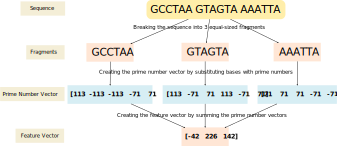
\includegraphics[width=\linewidth]{figures/PrimeNumberScoring.pdf}
  \caption{Example of feature extraction in the PNH}\label{fig:pnh}
\end{figure}

\subsection{Choice of primes for PNH}

The PNH provides a computationally light approach to extract features
from a nucleotide sequence.  Each of the $p$ dimensional features
embody nucleotide frequencies which is sensitive to biologically
meaningful features such as: direct repeats, inverted repeats, and
skew patterns~\cite{hemert-18} but is insensitive to inversions.  This
is the intuition behind the usage of PNH.

The choice of prime numbers to encode nucleotide is a balance.  Small
prime numbers (such as 3, 17, 23, etc.) were avoided in an attempt to
increase the uniqueness of the feature values~\cite{ye-14}.
Conversely, very large values are not used to ensure that a few
differences do not skew the features.  The default values of $P_{A}$ =
113 and $P_{G}$ = 71 were identified via preliminary analysis on HIV
sequences~\cite{delgado-15} and were also used as guidance for the
prime number choices, but was not highly optimized for any particular
organisms' genome.  Moreover, smaller values permit the use of faster,
primitive datatypes without concerns about numeric overflows (within
reason) during summations (see Figure~\ref{fig:pnh}).

\subsection{Impact of hyperparameters}

The Prime Numbers-based Heuristic (PNH) involves two key
hyperparameters, namely -- \ding{182} the number of features $p$ used
for comparing two reads, and \ding{183} $\tau_{prime}$: the threshold
Euclidean distance used to decide if two reads are sufficiently
similar.  Currently, the value of $\tau_{prime}$ for a given reference
sequence is computed as the average Euclidean distance from a given
reference strain minus the standard deviation.

The number of $p$ features has been set to a default value of 4 based
on experimental results summarized in
Figure~\ref{fig:pri-qual}. Overall, the number of features $p$ does
not have a significant impact on the clustering quality -- \ie\/ NMI
and purity do not vary much.  However, as the number of features $p$
is increased the number of clusters increase due to too many
false-negatives as the reads are broken into too short fragments.
Moreover, the memory usage also increases due to the overhead of
storing the large features.  Consequently, in this study, we have set
the value of $p$ to be 4.

\begin{figure}[h]
  \begin{minipage}{\linewidth}
    \centerline{\includegraphics[width=\linewidth]{../charts/param_analysis/primes_features_quality.pdf}}
    \centerline{(a) Impact on quality}
  \end{minipage}
  \begin{minipage}{\linewidth}
    \centerline{\includegraphics[width=\linewidth]{../charts/param_analysis/primes_features_runtime.pdf}}    
    \centerline{(b) Impact on runtime}
  \end{minipage}
  \caption{Impact of varying number of PNH features $p$}\label{fig:pri-qual}
\end{figure}

